% -*- root: main.tex -*-
%-------------------------------------------------------------------------------
\chapterimage{chapter_head_8.pdf} 

%-------------------------------------------------------------------------------
\chapter{ROS 패키지 이용 방법}

%-------------------------------------------------------------------------------
\section{로봇 패키지}\index{로봇 패키지}

%-------------------------------------------------------------------------------
\subsection{로봇 패키지}\index{로봇 패키지}

ROS에서는 중요한 하드웨어로 로봇과 센서를 꼽고있다. 이들의 로봇과 센서는 각각 패키지 형태로 제공되고 있다. 일부는 윌로우게러지 및 유진로봇, 알데바란과 같은 로봇 기업이 제공하는 경우도 있지만, 대부분은  로봇 공학 전공의 대학 연구실, 개인 개발자들이 자체 개발한 ROS 패키지\footnote{ROS Wiki Robot, http://wiki.ros.org/Robots}를 제공하고 있다. 

로봇 패키지의 대표작이라고 한다면 단연 PR2와 터틀봇을 꼽을 수 있다. 

그 중, PR2는 ROS 개발을 담당했던 윌로우 게러지에서 연구용으로 개발한 모바일 베이스의 휴머노이드형 로봇이다. 지금도 다른 로봇들의 핵심적인 패키지는 PR2 패키지로부터 파생된 것을 많이 사용하고 있을 정도로 대표적 로봇 패키지이다. 

그리고 또 다른 대표적인 로봇은 터틀봇이다. 터틀봇은 PR2가 범용적이고 성능면에서 뛰어나지만 가격면에서 ROS의 활성화를 이룰수 없다는 판단하에 ROS 의 활성화를 목적으로 한 개발용 모바일 로봇이다. 처음에는 iRobot 사의 청소로봇 룸바를 모바일 베이스로 채택했었고, 이어서 터틀봇2에서는 우리나라의 유진로봇사의 아이클레보를 개량한 거북이(KOBUKI) 를 모바일 베이스로 채택하여 지금까지 많이 사용되고 있다.

\begin{figure}[h]
\centering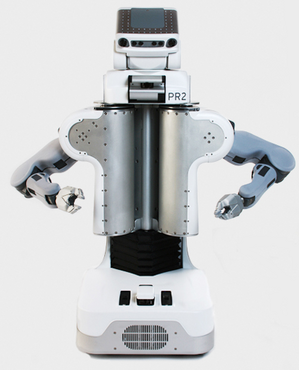
\includegraphics[height=55mm]{pictures/chapter8/PR2.png}
\centering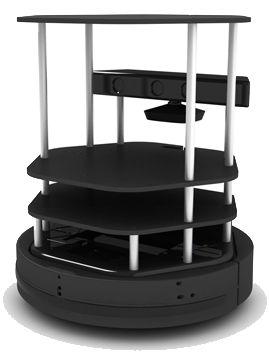
\includegraphics[height=55mm]{pictures/chapter8/turtlebot2.png}
\caption{좌측:PR2(http://www.willowgarage.com]), 우측:Turtlebot2(http://turtlebot.com)}
\end{figure}

\vspace{\baselineskip}
\noindent
이 대표적인 두 가지의 로봇 이외에도 120여 종류의 로봇이 소스를 제공하고 있다.  이는 오픈소스로 ROS 패키지 소스가 공개된 로봇들의 숫자이고, 로봇 관련 회사, 연구소, 대학, 개인 들이 사용하고 있는 로봇들의 수까지 합친다면 더 많을 것이라고 생각된다.

\begin{figure}[h]
\centering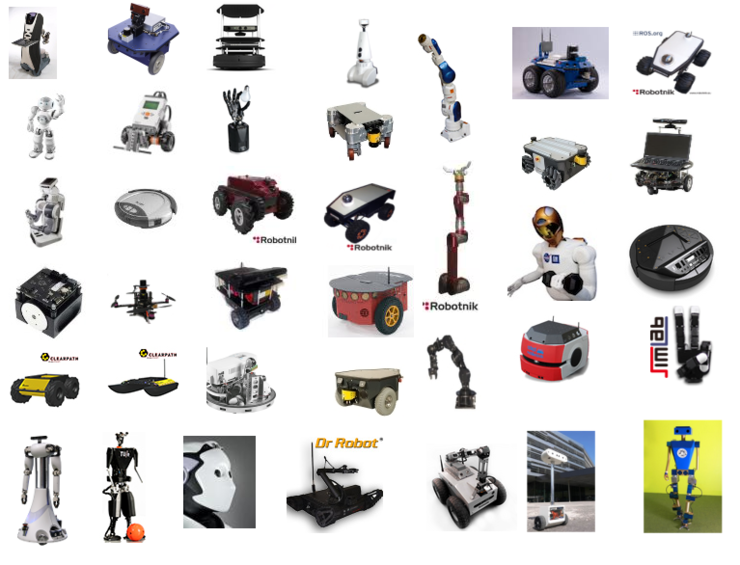
\includegraphics[width=\columnwidth]{pictures/chapter8/robots.png}
\caption{ROS가 도입한 로봇들 (http://wiki.ros.org/Robots)}
\end{figure}

로봇의 종류로는 아래와 같이 거의 모든 종류의 로봇 분류에서 사용되는 로봇들이 등록되어 있다. 공개된 로봇 패키지는 \url{http://wiki.ros.org/Robots} 에서 확인해 볼 수 있다.

\begin{itemize}[leftmargin=*]
\item 매니퓰레이터 (Manipulator)
\item 모바일 로봇 (Mobile robot)
\item 자동 주행 자동차 (Autonomous car)
\item 휴머노이드 (Humanoid)
\item 무인 항공기 (UAV: Unmanned Aerial Vehicle)
\item 무인 잠수함 (UUV: Unmanned Undersea Vehicle)
\item 무인 표면 주행차 (UWV: Unmanned Surface Vehicle) 
\end{itemize}



%-------------------------------------------------------------------------------
\subsection{로봇패키지 사용 방법}\index{로봇패키지 사용 방법}

만약, 사용하고자 하는 로봇 패키지가 ROS 공식 패키지라면 설치 방법은 매우 간단하다. 우선, 자신이 사용하고자 하는 로봇 패키지가 공개 되었는지 ROS wiki robot (\url{http://wiki.ros.org/Robots}) 에서 확인하거나 아래의 명령어로 전체의 ROS 패키지로부터 찾아 볼 수 있다.

\begin{lstlisting}[language=ROS]
$ apt-cache search ros-indigo
\end{lstlisting}

필자는 위 명령어보다 리눅스의 GUI 패키지 매니저 프로그램인 synaptic 을 구동하여  "ros-indigo" 으로 검색해볼 것을 추천하고 싶다. 사용하고자 하는 로봇 패키지가 공식 패키지라면 제일 간단하다. 아래의 그 예를 몇개 알아보기로 하곘다.

\vspace{\baselineskip}
\textbf{(예제1) PR2\footnote{ROS Wiki PR2, http://wiki.ros.org/Robots/PR2}}
PR2 경우는 아래의 명령어로 일괄 설치된다.
\begin{lstlisting}[language=ROS]
$ sudo apt-get install ros-indigo-pr2-desktop
\end{lstlisting}

\textbf{(예제2) 터틀봇2\footnote{ROS Wiki Turtlebot, http://wiki.ros.org/Robots/TurtleBot}}
터틀봇2의 경우는 아래와 같으며, 설치관련 wiki 페이지를 보고 몇가지 설정해주면된다.
\begin{lstlisting}[language=ROS]
$ sudo apt-get install ros-indigo-turtlebot ros-indigo-turtlebot-apps ros-indigo-turtlebot-viz ros-indigo-turtlebot-simulator ros-indigo-kobuki-ftdi
\end{lstlisting}

\textbf{(예제3) Nao\footnote{ROS Wiki NAO, http://wiki.ros.org/nao/Installation}}
Nao의 경우는 아래와 같으며, 설치관련 wiki 페이지를 보고 몇가지 설정해주면된다.
\begin{lstlisting}[language=ROS]
$ sudo apt-get install ros-indigo-nao-robot ros-indigo-nao-pose ros-indigo-nao-msgs ros-indigo-nao-driver ros-indigo-nao-description ros-indigo-nao-bringup ros-indigo-humanoid-nav-msg
\end{lstlisting}

만약에 해당 로봇 패키지가 공식적으로 제공되지 않더라도 로봇 패키지 위키에는 설치 방법등을 따로 설명해주고 있다. 예를들어 모바일 로봇으로 유명한 파이오니어(Pioneer)\footnote{ROS Wiki ROSARIA, http://wiki.ros.org/ROSARIA}의 경우, 아래와 같이 캐킨 빌드 시스템의 사용자 소스 폴더로 이동한 후, 위키에 적혀진 소스 리포지토리로부터 최신의 로봇 패키지를 다운로드 받으면 된다. 

\vspace{\baselineskip}
\begin{lstlisting}[language=ROS]
$ cd ~/catkin_ws/src %*(캐킨 빌드 시스템의 사용자 소스 폴더로 이동)*)
$ hg clone http://code.google.com/p/amor-ros-pkg/ %*(위키에 개재된 리포지토리로부터 소스 다운로드)*)
\end{lstlisting}

이와 같이, 공개된 로봇 패키지는 ROS 공식 패키지를 설치하던가, 위키 패키지에 적혀진 설치 방법에 따라, 공개 소스 리포지토리로부터 다운로드 후, 빌드 과정을 거치고 사용하면된다. 패키지안의 각 노드들의 사용설명은 해당 로봇 패키지의 설명을 따르기 바란다.

로봇 패키지는 기본적으로 로봇 구동 드라이브 노드, 장착된 센서 데이터의 취득 및 활용 노드, 원격 조정 노드, 관절형인 경우에는 역기구학 구동 노드, 모바일 로봇의 경우는 네비게이션 노드 등이 포함되어 있다. 


\newpage
%-------------------------------------------------------------------------------
\section{센서 패키지}\index{센서 패키지}

%-------------------------------------------------------------------------------
\subsection{센서}\index{센서}

로봇하면 떼어놓을 수 없는 것이 센서이다. 필자 또한 로봇관련 연구를 하고는 있다고 하지만, 주된 연구는 로봇에게 환경 정보를 전달하기 위하여 임베디드 센서를 환경측에 설치하고, 수 많은 환경 정보중에서 의미있는 환경 정보만을 추출 하여 인터넷을 경우하여 로봇이 필요로 할때 제공해주는 연구를 진행중이다. 

이러한 환경 정보로는 로봇의 위치, 장애물의 위치, 사람의 위치, 가구의 위치 등의 움직이는 사물에 대한 위치 정보도 있고, 방, 건물의 2차원, 3차원 지도 정보, 온/습/조도 정보, 날씨정보, 방안의 물건의 위치 및 물건 인식, 사람의 행동(제스쳐), 음성, 로봇 및 사물의 관성 정보, 토크정보, 진동, 가스, 소리, On/Off, 풍향 및 풍속, 사용 전류량, RFID 인식 등 정말로 다양하고 이러한 정보는 로봇이 작업을 수행하는데 사용된다.

이처럼, 로봇은 구동용 바퀴나 로봇 암을 달아 움직임을 만들었다고 로봇이 아니다. 여기서 그친다면 단순히 움직이는 기계를 만들어낸것에 불과하다고 볼 수 있다. 로봇은 로봇의 주변 환경을 인식하고 의미있는 정보만을 추출하여 사고 판단을 할 수 있을때 비로서 로봇이라고 볼 수 있다. 

이러한 환경 정보를 취득하기 위한 센서의 종류는 매우 많다. 그 중 로봇이 사용하는 대표적인 센서에는 거리 센서를 들 수 있다. LRF(Laser Range Finders) 및 적외선 거리센서가 가장 일반적이고, 최근에는 3D Sensors 인 키넥트, Xtion 등이 거리센서로서 많이 사용되고 있다. 그 이외에도 유저 인식, 물체 인식 등에 사용되는 컬러 카메라, 위치 추정에 쓰이는 관성센서, 음성인식에 사용되는 마이크폰, 토크 제어에 사용되는 토크센서 등 센싱해야 하는 정보에 대응하는 다양한 센서들이 존재한다.

아래의 그림은 ROS를 이용한것은 아니지만 필자의 연구실을 LRF 센서로 계측한 예제이다. ROS의 2D range finders 계열의 LRF 및 3D Sensors 를 이용하면 아래와 같은 결과물도 만들어 낼 수 있다.

\begin{figure}[h]
\centering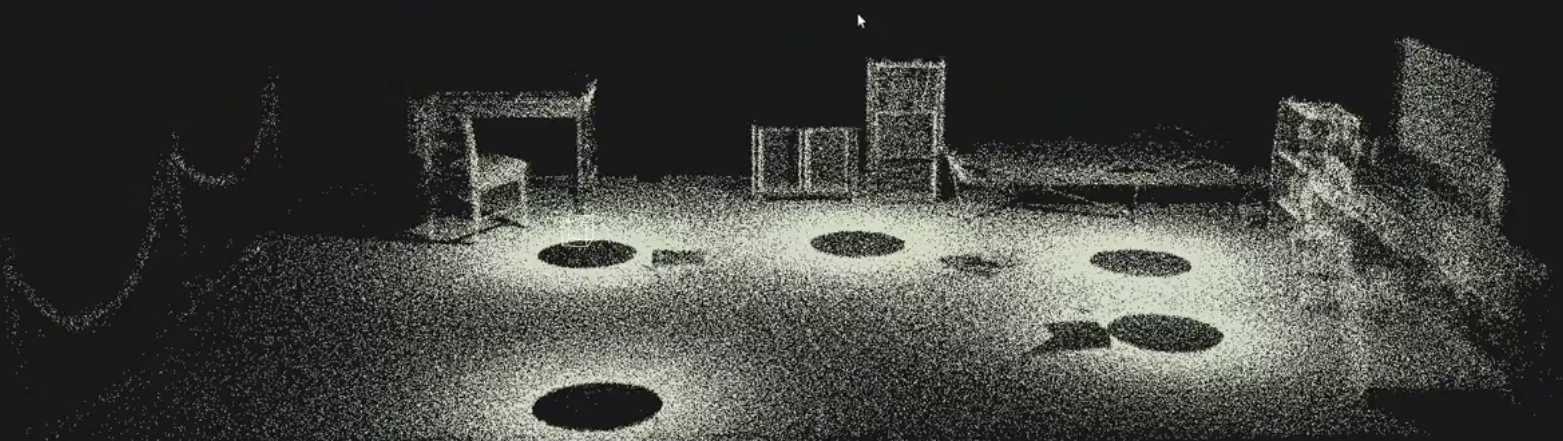
\includegraphics[width=\columnwidth]{pictures/chapter8/lrf360.png}
\caption{레이저 레인지 파인더로 만들어낸 3차원 지도}
\end{figure}

문제는 사용해야하는 센서는 정말 많다는 것이다. 단순히, 마이크로 프로세서에서 ADC로 값을 받을 수 있는 센서는 한계가 있다. 그 중 LRF, 3D Sensors, 카메라 등은 데이터 량이 많고, 처리에 상당한 스펙이 필요하기에 마이크로 프로세서로는 무리이고, PC를 이용하게 된다. 이에 따라 드라이버도 필요하고 OpenNI, OpenCV 등 포인트 처리, 영상 처리 등에 필요한 라이브러리도 필요하다.

ROS 는 위에서 언급한 센서들의 드라이버, 라이브러리 사용 가능한 환경 등을 제공해주고 있다. 현재 모든 센서를 제공하는 것은 아니지만 점점 센서관련 패키지는 늘어나고 있고, 사용법이 같은 센서 예를들어 I2C, UART 등을 사용한 센서들은 사용방법도 통일화되고 있다. 센서 제조회사들도 적극적으로 ROS 센서 패키지를 지원하고 있어서 향후 나온 센서들의 ROS 지원에도 가속화가 되지 않을까 싶다.

\begin{figure}[h]
\centering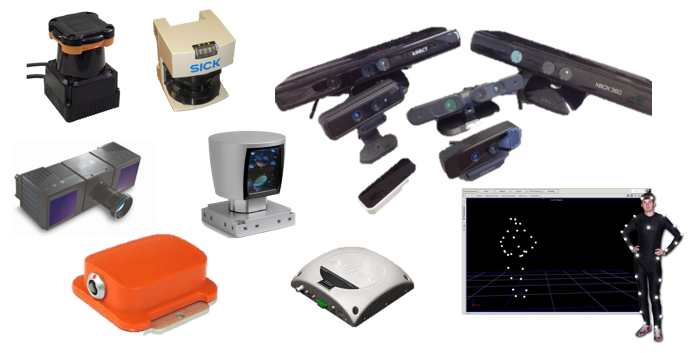
\includegraphics[width=0.8\columnwidth]{pictures/chapter8/sensors.png}
\caption{ROS에서 사용 가능한 센서의 예}
\end{figure}

%-------------------------------------------------------------------------------
\subsection{센서 패지키}\index{센서 패지키}

ROS 센서 위키 페이지\footnote{ROS Wiki, Sensors, http://wiki.ros.org/Sensors}에는 여러 센서 패키지를 공개되어 있다. 센서를 각 분류별로 1D range finders, 2D range finders, 3D Sensors, Pose Estimation (GPS+IMU), Cameras, Sensor Interfaces, Audio / Speech Recognition, Enviromental, Force/Torque/Touch Sensors, Motion Capture, Power Supply, RFID 등으로 구분되어 각 분류에 속하는 센서들을 소개하고 있다. 센서 패키지 자세한 사용법은 \url{http://wiki.ros.org/Sensors} 를 참조하면 좋을 듯 싶다. 특히, 필자가 중요하게 생각하는 패키지는 다음과 같다.

\vspace{\baselineskip}
\begin{itemize}[leftmargin=*]
\item 1D range finders : 저가의 로봇을 만들떄 사용할만한 적외선 방식의 직선 거리 센서
\item 2D range finders : LRF 센서로써 네비게이션에 많이 사용되는 센서들을 모아 두었다.
\item 3D Sensors : 프라임센서 기반의 kinect, asus 뿐만 아니라 다양한 3차원 계측에 필요한 센서를 모아 두었다.
\item Audio/Speech Recognition : 현재 음성인식 관련 부분은 매우 적지만, 지속적으로 추가될 것으로 보인다.
\item Cameras : 물체인식, 얼굴인식, 문자판독 등에 많이 사용되는 카메라의 드라이버, 각종 응용 노드들을 모아두었다.
\item Sensor Interfaces : USB 및 웹프로토콜을 지원하는 센서는 매우 적다. 아직까지도 많은 센서들은 마이크로프로세서에서 쉽게 취득 가능한 센서가 많다. 이러한 센서의 경우, 마이크로프로세서의 UART 및 미니PC 계열에서 ROS와의 연결을 지원한다. 이러한 인터페이스를 소개하고 있다.
 \item 각자 프로젝트에 맞는 센서들을 찾아서 자신의 프로젝트에 적용해 보도록 하자. 만약, 드라이버가 지원되지 않는다면 직접 구현해야 하는데 이는 나중에 관련 강좌를 구성해 보겠다.
\end{itemize}

%-------------------------------------------------------------------------------
\subsection{센서 패키지를 이용한 예제}\index{센서 패키지를 이용한 예제}

일반 USB CAM의 경우, UVC을 지원하기에 ROS의 "uvc\_camera" 패키지\footnote{ROS Wiki, UVC Camera, http://wiki.ros.org/uvc\_camera}를 이용하면 된다. 우선, 아래의 명령어로 "uvc\_camera" 패키지를 설치하도록 하자.

\begin{lstlisting}[language=ROS]
$ sudo apt-get install ros-indigo-uvc-camera 
\end{lstlisting}

\noindent
USB CAM을 컴퓨터의 USB에 연결하고, 아래의 명령어로 uvc\_camera 패키지의 uvc\_camera\_node 노드를 구동하자.

\begin{lstlisting}[language=ROS]
$ rosrun uvc_camera uvc_camera_node
\end{lstlisting}

그 후, 아래의 명령어로 rqt를 구동후, 플러그인(Plugins) 메뉴에서 이미지 뷰(Image View)를 선택한다. 그 뒤 왼쪽 상단의 메시지 선택란을 "/image\_raw"를 선택하면 아래의 화면처럼 영상을 확인할 수 있다. 

\begin{lstlisting}[language=ROS]
$ rqt
\end{lstlisting}

영상처리는 "/image\_raw" 의 토픽정보를 메시지로 받고 OpenCV 라이브러리를 보면서 각자 목적에 맞게 영상처리하는 노드를 별도로 작성하면 된다.

%-------------------------------------------------------------------------------
\subsection{공개 패키지 사용법}

%-------------------------------------------------------------------------------
\subsection{공개된 ROS 패키지 사용하기}\index{공개된 ROS 패키지 사용하기}

ROS 에 공개된 패키지가 얼마나 될까? 정확히는 몰라도 수천개는 될 것이다. 개발자가 ROS wiki 에 공개한 것과 wiki 에는 공개하지 않았지만 github 등에 공개한것까지 합치면 5000개는 족히 될 것이라고 추측된다. 그럼, 실제로 개발자가 ROS wiki 에 공개한 패키지를 알아보도록 하자.

우선, http://www.ros.org/browse/list.php 으로 가보도록 하자. 그러면 수많은 패키지 리스트가 보일 것이다. 그 중에서 아래 그림처럼 ROS의 최신 버전인 hydro 를 선택하고 밑의 packages 를 선택해주자. 그러면 아래 패키지 리스트가 끝도 보이지 않게 나열 되는 것을 볼 수 있다. 이 패키지가 ROS Hydro 버전으로 공개된 패키지이다. 대략 계산해보니  870여개가 된다. 이전 버전인 Groovy 의 경우는 1920여개, 가장 널리 쓰였던 Fuerte는 무려 2720여개의 공개된 패키지를 확인해 볼 수 있다. 참고로 각 버전간에 동일한 패키지가 있는 것은 업그레이드 되어도 노드도 함께 업데이트 되어서 이다.

그리고, ROS는 버전이 달라도 어느정도 호환성이 있기때문에 위의 공개된 패키지를 맘껏 이용가능하다.그렇다면 우리는 어떻게 이 패키지들을 사용할 수 있을까? 앞으로 이에 대해서 알아보도록 하자.

\begin{figure}[h]
\centering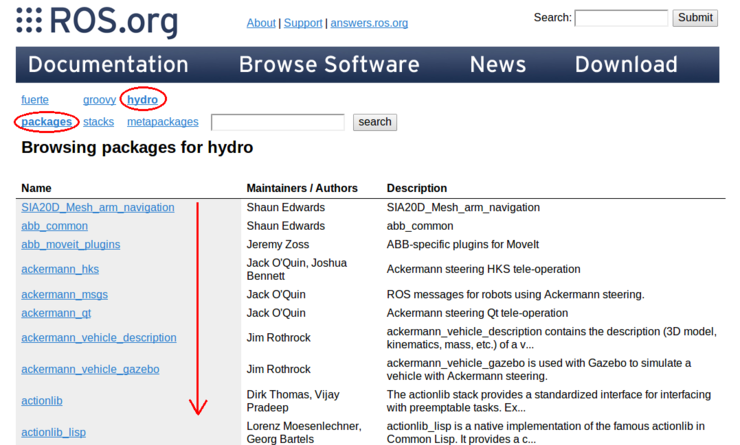
\includegraphics[width=0.9\columnwidth]{pictures/chapter8/openpkg1.png}
\caption{ROS 패키지 목록}
\end{figure}

%-------------------------------------------------------------------------------
\subsection{패키지 검색}\index{패키지 검색}

우리는 이 강좌에서 공개된 패키지를 사용해보는 것이였다. 뭔가 하나의 예제를 골라야하기 때문에 필자는 USB 카메라를 이용하여 얼굴 인식을 해보려고 한다. OpenCV를 이용하여 직접 만들어도 되곘지만 기존것이 있다면 가져다 쓰면 자신의 주력해야할 일에 집중할 수 있어서 더 좋지 않나 싶다.

그럼, 얼굴 인식과 관련된 용어로 검색해보자. 필자는 "face detect" 로 검색을 해보았다.

\begin{figure}[h]
\centering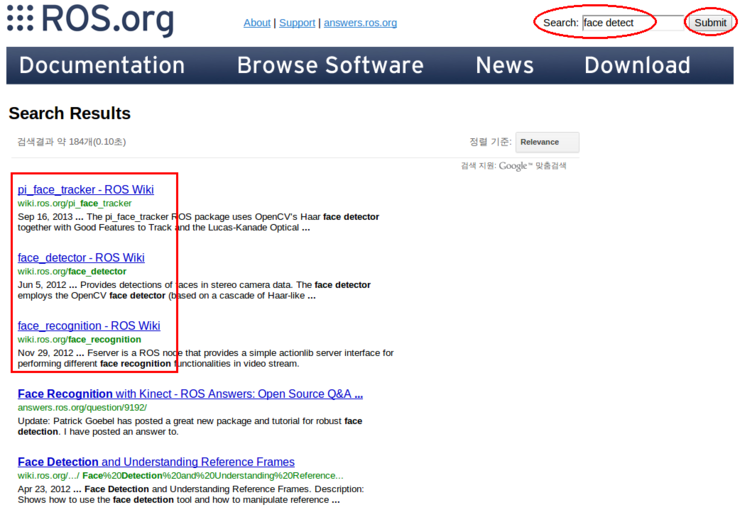
\includegraphics[width=0.9\columnwidth]{pictures/chapter8/openpkg2.png}
\caption{패키지 검색 방법}
\end{figure}

검색어가 적절하다면 위와 같이 관련 패키지가 상당히 검색된다.  우선, 가장 상단부의 pi\_face\_tracker 와 face\_detector 패키지가 가장 근접해 본다. 자세한 패키지 내역을 알기위해 각 wiki 페이지를 읽어보기 바란다. 필자는 처음에 face\_dector (http://wiki.ros.org/face\_detector) 를 선택했으나 패키지 설명 부분에서 kinect 및 Xtion과 같은 RGBD 카메라가 필요하다는 것을 확인하였고, 본래 목적인 USB 카메라로 사용할 수 없는 패키지이기에 단념했다.

그 뒤, pi\_face\_tracker 를 검색해보니 매우 쓸만해 보였고 이 패키지를 사용하기로 결정했다. 안되면 다른 패키지를 찾으면 그만이거나 이 패키지를 참고삼아 제작하면 그만이다. 단, 주의할 것은 catkin 인지 rosbuild 인지 알아두는것이 좋고, 누가 제작하였는지, 오픈소스 라이선스는 어떤것을 채택하고 있는지 꼭 유심히 체크해봐야 한다.

\begin{figure}[h]
\centering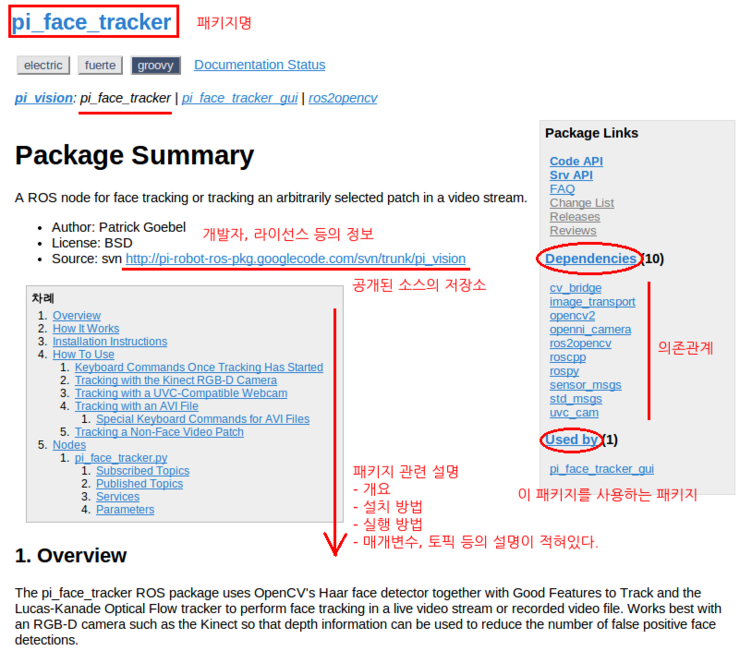
\includegraphics[width=0.9\columnwidth]{pictures/chapter8/openpkg3.png}
\caption{패키지 정보}
\end{figure}

그리고 난 후, 패키지의 오픈소스 저장소 주소, 패키지 의존관계 등을 필히 숙지한다. 패키지를 설치하기 전에 의존하는 패키지는 우선적으로 설치를 해줘야만 해당 패키지를 사용할 수 있다. 그럼 다음 챕터에서 직접 설치해보자.

\newpage
%-------------------------------------------------------------------------------
\subsection{패키지 설치}\index{패키지 설치}

\begin{figure}[h]
\centering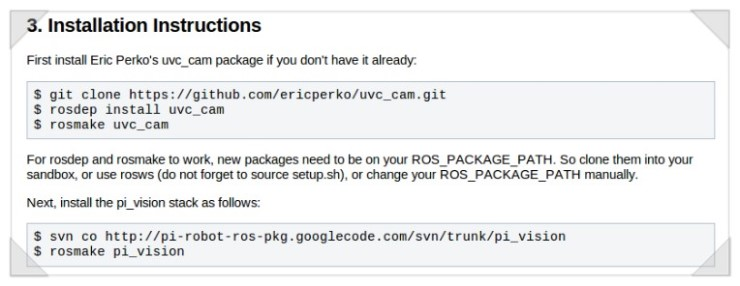
\includegraphics[width=0.9\columnwidth]{pictures/chapter8/openpkg4.jpg}
\caption{패키지 설치}
\end{figure}

우선, 제일 먼저 wiki 페이지에서 설치관련 정보를 확인하자. 위 설치 과정에서는 uvc\_cam 와 pi\_vision 두 가지 패키지를 설치하도록 되어 있는데 자세히 보니 현재 hydro 에서 채택하고 있는 catkin 빌드 시스템이 아닌 rosbuild 빌드 시스템의 빌드 명령어인 rosmake 가 사용되고 있음을 확인할 수 있다. 가끔씩 이렇게 이전 빌드 시스템을 사용하고 있는 오래된 패키지가 있다. 하지만 그렇다고 해서 설치 불가능 한것이 아니라 hydro 에서는 catkin 과 rosbuild 를 모두 사용할 수 있기 때문에 문제가 없다.

예제대로 설치해주도록 하자. 참고로 git clone 명령어는 다음의 주소의 저장소의 소스코드를 전부 다운로드 하라는 명령어이며, rosdep install uvc\_cam 은 uvc\_cam 패키지의 의존선 패키지를 미리 설치하라는 명령어이다. 그리고 마지막으로 rosmake uvc\_cam 는 uvc\_cam 를 빌드하여 실행 파일을 생성하라는 명령어이다.

\vspace{\baselineskip}
\begin{lstlisting}[language=ROS]
$ git clone https://github.com/ericperko/uvc_cam.git
$ rosdep install uvc_cam
$ rosmake uvc_cam
\end{lstlisting}

그 다음, 아래의 pi\_vision 패키지를 설치해보도록 하자. 실제로 해본 사람은 알겠지만 중간에 빌드가 멈추고 에러가 발생하는데 rosbridge 가 없다고 나온다.  이는 "sudo apt-get install ros-hydro-rosbridge-server" 명령어로 설치해주면 끝날 것이라고 생각되지만 pi\_vision 는 rosbridge 의 1.0 을 요구하고 있어서 현재의 hydro 및 groovy 에서는 rosbridge 2.0 만 제공하고 있어서 설치가 불가능하다. pi\_vision 버전이 상당히 오래된것으로 생각된다.

\vspace{\baselineskip}
\begin{lstlisting}[language=ROS]
$ svn co http://pi-robot-ros-pkg.googlecode.com/svn/trunk/pi_vision
$ rosmake pi_vision
\end{lstlisting}

다만, pi\_vision 은 roscpp가 아닌 python 으로 작성되었기 때문에 패키지의 srv 및 msg 만 빌드하여 생성해주면 이용 가능하다.  아래의 명령어로 메시지 및 서비스만 빌드하자.

\vspace{\baselineskip}
\begin{lstlisting}[language=ROS]
$ roscd pi_face_tracker
$ make
\end{lstlisting}

이로써 얼굴 인식에 필요한 모든 패키지를 설치하였다. 만약에 그 이외에 의존 패키지로 문제가 된다면 위에서 설명하였던 패키지의 의존 패키지인 cv\_bridge, image\_transport, opencv2, openni\_camera, ros2opencv, roscpp, rospy, sensor\_msgs, std\_msgs, uvc\_cam 가 설치 되어있는지 체크해봐야 할 것이다.

%-------------------------------------------------------------------------------
\subsection{패지키의 노드 실행}\index{패지키의 노드 실행}

\begin{figure}[h]
\centering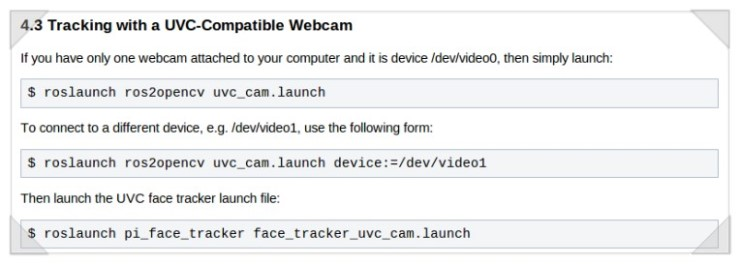
\includegraphics[width=0.9\columnwidth]{pictures/chapter8/openpkg5.jpg}
\caption{패지키의 노드 실행}
\end{figure}

일단, 위와 같이 패키지의 실행 방법을 확인하자. 그리 어려움은 없고 roslaunch 로 실행 가능하다. 그럼 우선, roscore 를 구동하고, 참고로 roscore는 앞으로 부터는 항상 구동해두는 습관을 가지도록 하자. 다음 부터는 별도로 설명하지 않겠다. 그 뒤, 별도의 다른 터미널 창을 열어 아래의 명령어로 카메라 드라이버를 구동하자.

\vspace{\baselineskip}
\begin{lstlisting}[language=ROS]
$ roslaunch ros2opencv uvc_cam.launch
\end{lstlisting}

\noindent
이번에는 다른 터미널 창을 다시 열어서 아래의 명령어로 얼굴 인식 노드를 구동하자.

\vspace{\baselineskip}
\begin{lstlisting}[language=ROS]
$ roslaunch pi_face_tracker face_tracker_uvc_cam.launch
\end{lstlisting}

지금까지 문제가 없었다면 아래 영상과 같이 얼굴의 몇가지 특징점을 찾아 얼굴 인식이 되는 결과를 확인할 수 있다. 아 그리고 참고로 터미널 창에서 rostopic echo /roi 라고 명령하면 현재 얼굴의 좌표점이 출력된다. 나중에 이 패키지를 이용하여 자신만의 패키지를 작성할 때 이 좌표를 받아 응용 노드를 작성할 수도 있다.

\begin{figure}[h]
\centering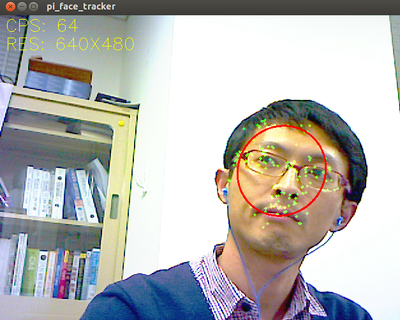
\includegraphics[width=0.5\columnwidth]{pictures/chapter8/openpkg6.png}
\caption{pi\_face\_tracker 실행 결과}
\end{figure}

ROS 에 공개된 패키지는 ROS가 널리 사용되기 시작하면서 급격히 증가하고 있다. 그 중 우리가 필요할 때 찾아쓰는 방법만 알아두면 미리 고민하고 노력해준 이들로 인하여 나의 작업은 한 단계를 넘어서서 내가 진정 집중해야할 부분에 시간을 쏟을 수 있게 된다. 이게 바로 ROS 의 기본 이념이다. 지식이 점점 쌓여져 더 상위단계로 접근하게 하여 로보틱스의 발전을 가져오는 것이다.







